\section{Proposed Approach}

This section gives the details about our proposed method which aims at detecting counterfeit fingerprints from applications' outbound HTTP traffics. Before going further, all PCAP files collected by an enterprise's host is network activities generated by a set of applications such as browsers $B = \begin{Bmatrix} b_{1}, & ... & , b_{n} \end{Bmatrix}$, and which are all installed in hosts. Each browser $b_{i}$ has several PCAP files which contain specific network characteristics, and our proposed approach possibly create a fingerprint $f_{b_{i}}$ for each browser. The PCAP files of a host $H$ include union of all browser fingerprints which is defined as $H = \cup^{n}_{j} f_{b_{i}}$. The proposed counterfeit fingerprint detection process consists of training and testing phases. In training phase, we assume enterprise hosts aren't compromised. This method mainly arises from the first one that is a data-driven and unsupervised flow responsible for a browser's fingerprint \cite{bortolameotti2017decanter} and referrer correlation construction. This step takes the fields of a PCAP file as input and classifies browser traffics, and then construct fingerprints and referrer correlation graphs. In the testing phase, given a browser outbound HTTP traffic reconstructed by fingerprint and referrer correlation graph, and the second step filters benign browser traffics through fingerprint matching. Continuously, compare its and trained referrer correlation graph using Graph Edit Distance (GED) for counterfeit fingerprint detection. The proposed method is depicted in figure \ref{fig:sa} and following paragraphs describe the details of each component.

\begin{figure*}[!t]
\centering
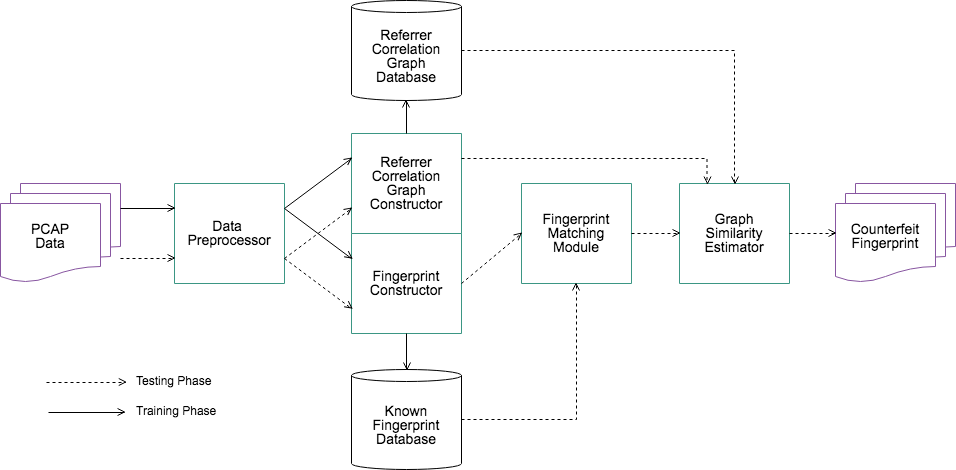
\includegraphics[width=400pt]{image/sa.png}
\caption{An overview of our counterfeit fingerprint detection system. Five subsystems are depicted: (1) data preprocessor subsystem, (2) fingerprint constructor subsystem, (3) fingerprint matching subsystem, (4) referrer correlation graph constructor subsystem, and (5) graph similarity estimator subsystem. The system only takes the PCAP files of outbound HTTP traffics as input. In training phase, subsystem (1) and (2) passively extract the benign fingerprint from an application's outbound HTTP traffic, and subsystem (3) could use fingerprints to classify benign traffic in the testing phase. We note that referrer correlation extraction in the subsystem (4) is a key step, in the sense that if it can extract discriminative features for counterfeit fingerprint detection, the detection in the subsystem (5) is relatively straightforward.}
\label{fig:sa}
\end{figure*}

\subsection{Browser Traffic Extractor}

For most cases of client-side attacking, hackers whose general goal is to steal valuable data before malware connects to C\&C server. As a result, PCAP files, that contain specific network characteristics of an application (e.g., browser) for each host in the enterprise. 

To generate fingerprint for each browser, our approach first extracts various entities from PCAP files. Table~\ref{tbl:log_01} shows 6 heterogeneous fields which can be extracted from each one-line log, including domain ({\em Domain}), destination IP ({\em DstIP}), user-agent ({\em User-agent}), accept language ({\em Accept-Lang}), length ({\em Len}), and constant field ({\em Constant}). The reason for choosing these 6 fields for browser traffic classification can be summarized as followings and fingerprint construction is represented in next subsection.

\begin{table}[]
\centering
\caption{Fields and Values of Database in a PCAP File}
\label{tbl:log_01}
\begin{tabular}{ll}
\hline\hline
Field                           & Value for Instance                                               \\\hline
{\em Domain}            & yahoo.com.tw                                                      \\
{\em DstIP}                & 140.92.88.140                                                     \\
{\em User-agent}      & Mozilla/5.0 (Windows NT 6.1; Win64; x64) ...  \\
{\em Accept-Lang}   & zh-TW                                                                  \\
{\em Len}                   & 1253                                                                     \\
{\em Constant}          & If-Modified-Since, Cookie, Connection, ...       \\\hline\hline
\end{tabular}
\end{table}

In previous research \cite{bortolameotti2017decanter}, Bortolameotti et al. identified two types of HTTP applications (e.g., $browser$ and $background$). This subsection aims to filter logs of a PCAP file according to the {\em User-agent}, because we focus on counterfeit fingerprints of browser network activities. To identify browser activities, the browser flags we defined are "Mozilla", "Opera", "MQQBrowser", "UCWEB",  "NOKIA5700", "Openwave", "Safari", and "Chrome", and which are used for string matching in field {\em User-agent}. Furthermore, in both training and testing phase, an implementation time-slot $t$ is a fixed time window of $T$ minutes, and the filtered logs is passed to the next module after $t$ ends.

\subsection{Fingerprint Constructor}

\subsection{Fingerprint Matching Module}

\subsection{Referrer Correlation Graph Constructor}

\subsection{Graph Similarity Estimator}

We denote the graph edit distance between two opcode-component graphs $g_{1}$ and $g_{2}$ as $D(g_{1}, g_{2})$, which is the sum of VertexCost and EdgeCost. In which, VertexCost and EdgeCost indicate the numbers of insertions, deletions and substitutions of vertices and edges, respectively, where determine the minimum amount of distortion for transforming one graph into another graph  \cite{p:Fankhauser11}. Let $g_{1}$ = $(V_{1}, E_{1})$  and $g_{2}$ = $(V_{2}, E_{2})$: $g_{1}$ is the source graph of malware, and $g_{2}$ is the target graph of malware. The graph edit distance between $g_{1}$ and $g_{2}$ is defined as follows:

\begin{equation}
        \label{eq:ged}
        D(g_{1}, g_{2}) = \mathbf{VertexCost} + \mathbf{EdgeCost}
\end{equation}

\begin{equation}
        \label{eq:cost_all1}
\sigma (g_{1},g_{2}) = \frac{D(g_{1}, g_{2})}{\left | V(g_{1}) \right | + \left | V(g_{2}) \right | +\left | E(g_{1}) \right | + \left | E(g_{2}) \right |}
\end{equation}

Finally, the similarity $\sigma (g_{1},g_{2}) $ of two graphs $g_{1}$ and $g_{2}$ is obtained from the graph edit distance $D(g_{1}, g_{2})$. The details are described in Equation~\ref{eq:cost_all1}, which is a real value on the interval [0,1], where 0 indicates that graphs $g_{1}$ and $g_{2}$ are identical, whereas a value near 1 implies that the pair is highly dissimilar. As mentioned before, finding the minimum graph edit distance, i.e., $min_{D(g_{1}, g_{2})}$, is an NP-hard problem but can be approximated. Riesen et al. and  Francesc Serratosa introduced an approximation algorithm with a good trade-off between accuracy and speed \cite{p:Riesen09} \cite{p:Serratosa14}. Given two graphs $G_{1}$ and $G_{2}$, where $\mid G_{1}\mid$ = n and $\mid G_{2}\mid$ = m, their algorithms, respectively, use a $(n+m) \times (n+m)$ cost matrix $C_{1}$ and a $n \times m$ cost matrix $C_{2}$, which both give the cost of mapping a vertex $v \in V(G_{1})$ to a vertex $v \in V(G_{2})$. Next,  Munkres algorithm \cite{p:Munkres57}, also known as the Hungarian algorithm, which runs in polynomial time, is applied to find an exact one-to-one vertex assignment  that minimizes the total mapping cost. Each entry in the cost matrix represents the cost of matching vertex $v \in V(G_{1})$ to a vertex $u \in V(G_{2})$. The cost of matching a pair of nodes $c_{ij}$ could equal the transformed cost as defined for the graph edit distance in the following subsection.

In this subsection, more accurate cost estimation allows the discovery of better graph matchings and hence more accurate edit distances.  The cost of matching a pair of vertices, element $c_{ij}$ of the matrix, could equal the transformed cost as defined for the graph edit distance, which consists three components:  Host jaccard similarity, In-degree,  jaccard similarity and  Out-degree jaccard similarity can be observed developing between vertices $v$ and $u$ but can be presented as $\delta \left ( v, u \right )$, $\delta^{-} \left ( v, u \right )$ and $\delta^{+} \left ( v, u \right )$, and their details can be defined as follows: 

\begin{equation}
        \label{eq:hostop}
 \delta \left ( v, u \right ) = \left | 1 - \frac{Bit_{op}\left ( v \right ) \cap Bit_{op}\left ( u \right )}{Bit_{op}\left ( v \right ) \cup  Bit_{op}\left ( u \right )} \right |
  \end{equation}
 
 \begin{equation}
        \label{eq:inop}
\delta^{-} \left ( v, u \right ) = \left | 1 - \frac{Neighbor^{-}\left ( v \right ) \cap Neighbor^{-}\left ( u \right )}{Neighbor^{-}\left ( v \right ) \cup  Neighbor^{-}\left ( u \right )} \right |
 \end{equation}
 
 \begin{equation}
        \label{eq:outop}
\delta^{+} \left ( v, u \right ) = \left | 1 - \frac{Neighbor^{+}\left ( v \right ) \cap Neighbor^{+}\left ( u \right )}{Neighbor^{+}\left ( v \right ) \cup  Neighbor^{+}\left ( u \right )} \right |
 \end{equation}
  
 where $Bit_{op}\left ( v \right )$ indicates the extraction of vertex $v$'s opcode components, presented by 218 binary bits defined as the above section. Additionally, $Neighbor^{-}\left ( v \right )$ and $Neighbor^{+}\left ( v \right )$ , respectively, present the Neighbor vertices of vertex $v$, which are defined as follows:
 
 \begin{equation}
        \label{eq:indegree}
Neighbor^{-}\left ( v \right ) = \left \{ z \mid e_{z,v} \in E \right \}
  \end{equation}
  
  \begin{equation}
        \label{eq:outdegree}
 Neighbor^{+}\left ( v \right ) = \left \{ z \mid e_{v,z} \in E \right \}
  \end{equation}
   
 Clearly, each element $c_{ij}$ of the cost matrix indicates the bijective mapping of the i-th vertex to the j-th vertex that can be defined as follows:
  
  \begin{equation}
        \label{eq:cost_element}
 c_{ij} = \delta \left ( i, j \right ) + \delta^{-} \left ( i, j \right ) + \delta^{+} \left ( i, j \right )
   \end{equation}

The Munkres algorithm \cite{p:Munkres57} \cite{p:Kuhn56} is a known algorithm that solves the bipartite matching problem in polynomial time. After obtaining the conceptual matched matrix,  we implement the Munkres algorithm to find the optimal permutation that minimizes the cost as the similarity distance between the two Android malicious samples' graphs $g_{1}$ and $g_{2}$. In Algorithm~\ref{alg:WBPAlgo}, the first three steps determine whether the cost matrix has the specific scenario which means the optimization bipartite match from source sample's vertex to target sample's vertex already exists. Then, we can decide whether the scope of the cost matrix needs to be reduced. Furthermore, we acquire a conceptual match matrix $C'$ from the function $f_{gm}(C)$, which can effectively eliminate the side-effects of each wide variability.
